% ============================================================
\chapter{Background and Related Work}
\label{ch:background}
% ============================================================

\section{Traversability as Perception of an Affordance}

Traversability estimation asks whether a mobile platform can move through a
region of the environment. This differs from semantic terrain recognition.
The class ``grass'', for example, does not determine whether the surface is
load-bearing, whether vegetation hides a ditch, or whether the slope exceeds
the vehicle's limits. Conversely, several semantic materials can form one
continuous traversable corridor. Surveys therefore describe traversability as
a combination of geometric, appearance-based, semantic, and
vehicle-interaction evidence~\cite{islam2022review,sevastopoulos2022survey}.

Geometric approaches use LiDAR, stereo, or structured depth to estimate slope,
roughness, steps, and obstacle height. They offer direct evidence for some
physical constraints, but flat vegetation, water, deformable soil, and sparse
returns remain difficult. Appearance-based systems use colour, texture, shape,
and learned context from RGB images. They are inexpensive and information-rich
but cannot reliably infer every physical property. A multimodal system can
combine both strengths at the cost of calibration, synchronisation, sensor
weight, and computation.

Another distinction concerns the source of supervision. Human annotation can
describe regions that appear suitable for a vehicle. Self-supervised systems
can learn from wheel slip, suspension response, vehicle tracks, or a geometric
teacher. Interaction-derived labels are platform-specific, but they cover only
terrain the robot visits and inherit the assumptions of the teacher signal.
The present study uses a human-annotated dataset because it enables every model
to receive exactly the same dense target. This makes architectural comparison
possible, while leaving the physical validity of the labels as an explicit
limitation.

\section{Off-Road Perception Datasets}

Off-road datasets vary in their task, sensors, geography, and label semantics.
RUGD supplies dense outdoor semantic labels in unstructured scenes
~\cite{wigness2019rugd}. RELLIS-3D combines RGB and LiDAR at an off-road
proving ground~\cite{jiang2021rellis}. TartanDrive emphasises multimodal
sequences and vehicle dynamics~\cite{triest2022tartandrive}. ORFD targets
off-road freespace detection with RGB and LiDAR-derived information
~\cite{min2022orfd}. WildScenes provides repeated natural-environment
traversals with calibrated image and LiDAR data, enabling 2D, 3D, and
domain-adaptation studies~\cite{vidanapathirana2025wildscenes}.

Table~\ref{tab:background_datasets} summarises the sensing modalities and label
scope of these datasets relative to the monocular binary task used here.

\begin{table}[H]
\centering
\caption{Representative off-road datasets and their relation to this work.}
\label{tab:background_datasets}
\small
\begin{tabularx}{\textwidth}{@{}lrrlX@{}}
\toprule
\textbf{Dataset} & \textbf{Year} & \textbf{Images} & \textbf{Primary data} & \textbf{Main label or research focus} \\
\midrule
RUGD~\cite{wigness2019rugd} & 2019 & 7,453 & RGB & 24 semantic outdoor classes \\
RELLIS-3D~\cite{jiang2021rellis} & 2021 & 6,235 & RGB + LiDAR & Multimodal off-road semantics \\
CaT~\cite{sharma2022cat} & 2022 & 1,812 & RGB & Nested vehicle-capability traversability \\
TartanDrive~\cite{triest2022tartandrive} & 2022 & --- & Multimodal & Terrain interaction and vehicle dynamics \\
ORFD~\cite{min2022orfd} & 2022 & 12,198 & RGB + LiDAR & Off-road freespace detection \\
WildScenes~\cite{vidanapathirana2025wildscenes} & 2025 & sequences & RGB + LiDAR & Natural-scene semantics and domain change \\
\bottomrule
\end{tabularx}
\end{table}

CaT is smaller than several alternatives, but its label semantics are
particularly relevant to the research question. Instead of assigning material
names, it represents nested vehicle capability: sedan-traversable terrain is
contained within pickup-traversable terrain, which is contained within
off-road-vehicle-traversable terrain~\cite{sharma2022cat}. This hierarchy can
be converted directly into different binary operating policies. Its small size
also makes data efficiency, pretraining, and overfitting central concerns.

\section{Dense Semantic Segmentation}

\subsection{From Image Classification to Pixel-Level Prediction}

A conventional image classifier answers one question about an entire image:
for example, whether the image contains a road vehicle. Semantic segmentation
answers a different and more detailed question. It assigns a class to every
pixel, so its output has the same spatial meaning as the input image. In the
binary task used in this thesis, each output pixel represents one of two
decisions: \emph{traversable} or \emph{untraversable}. The result can therefore
be displayed as a mask laid directly over the camera image.

This distinction changes the design of the network. A classifier is allowed to
discard the exact position of an object as long as it identifies the object
correctly. A segmentation model must retain enough position information to
reconstruct boundaries. If a trail occupies the centre of an image, predicting
``trail present'' is not sufficient; the model must indicate where the trail
begins and where the vegetation, ditch, or obstacle beside it starts.

The input to the models in this work is an RGB image. RGB means that each pixel
is represented by three numbers describing its red, green, and blue intensity.
The first layers of a convolutional neural network (CNN) apply small learned
filters across this image. A filter can respond to a simple local pattern such
as an edge, a colour transition, or a texture. Later layers combine many such
responses into more abstract features. A feature is not a manually assigned
label; it is an internal numerical representation learned because it helps the
network reduce its training error.

The region of the input that can influence one feature is called its
\emph{receptive field}. Early features see only a small neighbourhood. Deeper
features can see a much larger part of the scene. This larger view is useful:
a brown patch may be recognised as part of a track only after the network also
sees its continuation through the image. However, repeatedly reducing the
feature-map resolution to obtain this wider view also removes fine spatial
detail. Semantic segmentation architectures are largely different solutions
to this trade-off between broad context and precise location.

\subsection{The Encoder--Decoder Pattern}

The development of fully convolutional networks made it possible to train a
network end to end for dense prediction~\cite{long2015fcn}. ``Fully
convolutional'' means that the network does not end with the fixed-size
fully-connected classification layers used by older image classifiers.
Instead, it preserves a spatial grid of features and converts that grid back
into a pixel-level prediction.

Most modern segmentation systems can be explained using two components:

\begin{itemize}
  \item The \textbf{encoder} reads the image and progressively builds stronger
  semantic features. It commonly reduces width and height while increasing the
  number of feature channels. This makes processing cheaper and increases the
  receptive field, but it also produces a coarse representation.
  \item The \textbf{decoder} converts the coarse representation into a dense
  mask. It increases the spatial resolution and combines high-level meaning
  with earlier features that still contain local detail.
\end{itemize}

Increasing resolution is often called \emph{upsampling}. Upsampling alone
cannot recreate information that the encoder discarded. For this reason,
decoders frequently use \emph{skip connections}: direct routes that carry
features from an earlier, higher-resolution encoder stage to a corresponding
decoder stage. The decoder then has both kinds of evidence available. Deep
features help decide \emph{what} a region is, while shallow features help
decide \emph{where} its edge lies.

Figure~\ref{fig:segmentation_concept} summarises this complete change of
representation. The image is compressed into progressively coarser feature
grids, then expanded into a mask. The skip connections carry location detail
around the narrowest part of the network instead of asking the decoder to
invent that detail from the coarse representation.

\begin{figure}[H]
\centering
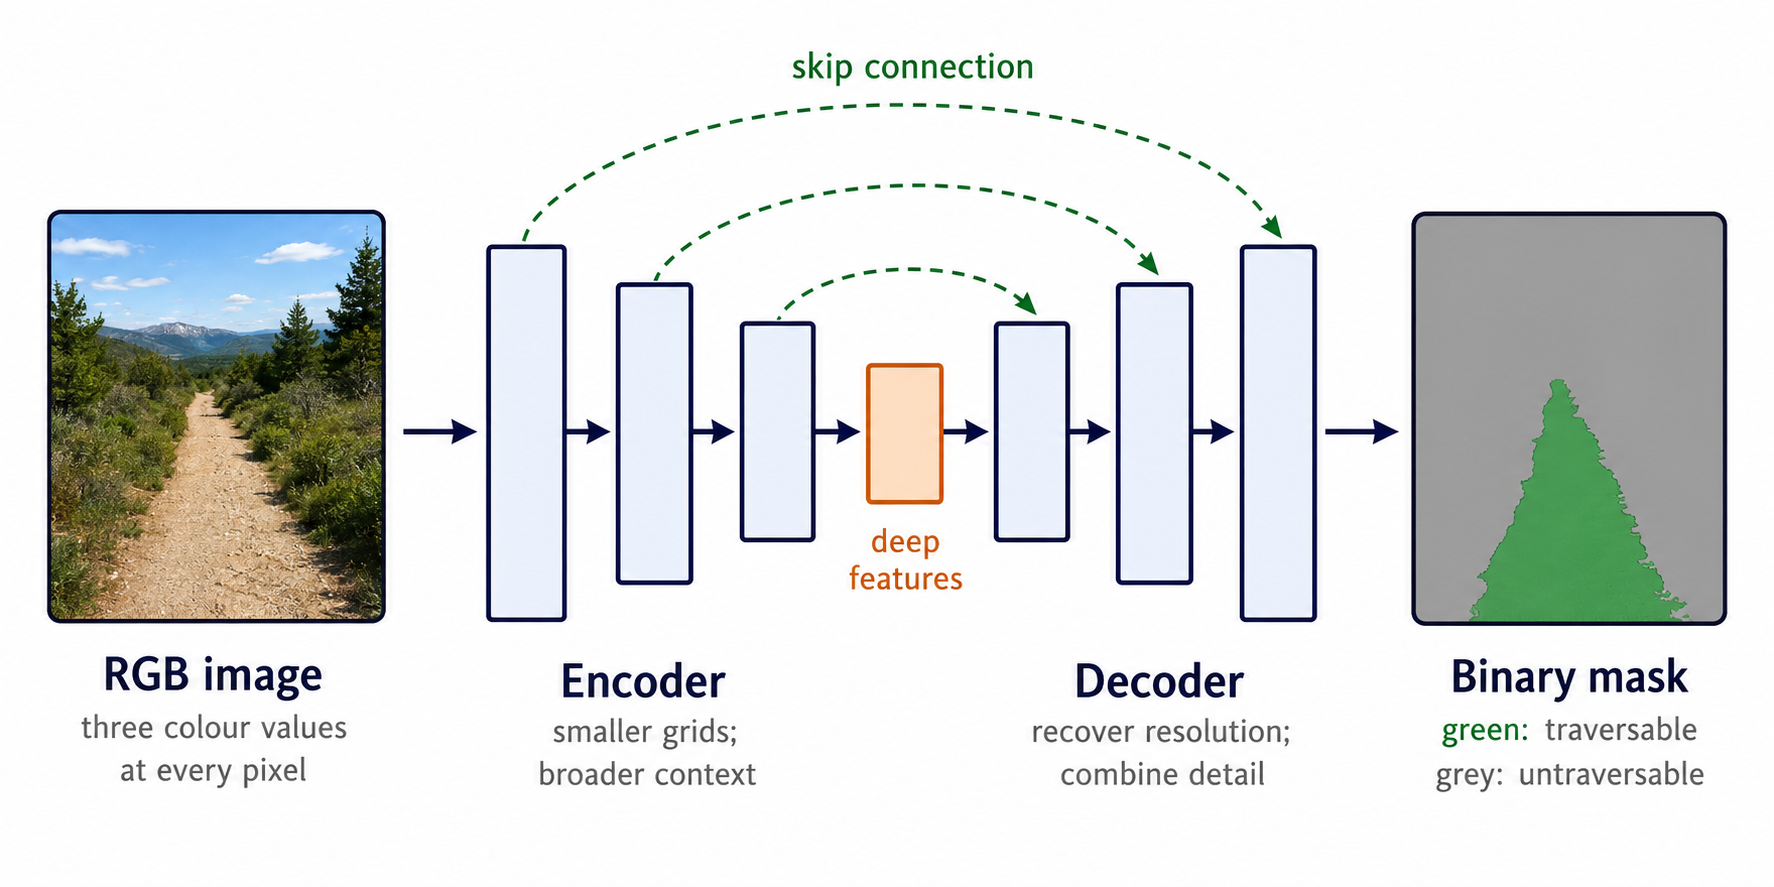
\includegraphics[width=\textwidth]{../fig2dash1.png}
\caption[From an RGB image to a binary segmentation mask.]{From an RGB image
to a binary segmentation mask. The encoder gathers increasingly broad context,
the decoder restores spatial resolution, and skip connections preserve local
detail. The landscape and mask are conceptual rather than dataset samples.
Original schematic drawn for this thesis.}
\label{fig:segmentation_concept}
\end{figure}

U-Net is a clear example of this pattern~\cite{ronneberger2015unet}. Its encoder
contracts the image representation in several stages, and its approximately
symmetric decoder expands it again. At each scale, a skip connection provides
the decoder with encoder features of the same resolution. U-Net was introduced
for biomedical images, where accurate boundaries are important, but the same
design principle is useful for roads, terrain, and many other segmentation
tasks.

Feature Pyramid Networks (FPNs) organise the same multi-scale idea
differently~\cite{lin2017fpn}. The encoder first produces a hierarchy of
features: fine features near the input and coarser, more semantic features
deeper in the network. A top-down path then carries semantic information back
towards the finer resolutions. Lateral connections join the top-down signal
with the encoder feature at each scale. The result is a pyramid in which
several resolutions contain useful semantic information. Although FPN was
introduced for object detection, this pyramid is also a practical decoder for
segmentation.

\subsection{Learning Context at More Than One Scale}

An object or terrain region does not have one fixed size in the image. Nearby
stones may occupy many pixels; the same stones in the distance may occupy only
a few. Segmentation systems therefore need to combine information gathered at
different spatial scales.

PSPNet does this using pyramid pooling~\cite{zhao2017pspnet}. It pools a deep
feature map into several grid sizes. A very coarse grid summarises almost the
whole scene, while finer grids retain more local variation. The pooled results
are resized and combined, giving the prediction access to both global and
regional context. DeepLabv3+ uses another method, known as \emph{atrous} or
\emph{dilated} convolution~\cite{chen2018deeplab}. A dilated filter samples
positions that are spaced apart, allowing it to cover a wider area without
reducing the feature-map resolution by the same amount. DeepLabv3+ then adds a
decoder to refine boundaries.

These methods are not merely interchangeable names. They express different
engineering choices. Pooling summarises regions explicitly. Dilated
convolution widens the sampled neighbourhood. Skip-connected decoders recover
detail from earlier layers. Multi-resolution networks, discussed below, keep
more than one resolution active throughout much of the model. Each choice
changes memory use, computation, and the type of spatial evidence that reaches
the final classifier.

\subsection{What the Network Produces in This Thesis}

The final layer produces one numerical score, or \emph{logit}, for each class
at each pixel. A logit is an unnormalised confidence value. During training,
the logits are compared with the annotated mask by a loss function. The loss
is a single number that measures how incompatible the prediction is with the
target; optimisation changes the network weights to reduce it. During
evaluation, the class with the stronger output is selected, or an equivalent
probability threshold is applied for the binary decision.

For CaT, the target is not a material map. The positive class is defined by a
vehicle-capability policy described in Chapter~\ref{ch:cat_pipeline}. A pixel
showing grass can be positive in one place and negative in another if the
annotation indicates different vehicle access. The network is thus learning a
visual approximation of the released capability labels, not a universal law
that grass, soil, or gravel is always safe.

The context--resolution trade-off has a direct meaning here. The model should
recognise that a partly shadowed surface continues as one track, which requires
scene context. At the same time, it should place the border between that track
and adjacent vegetation accurately, which requires local detail. A large open
region contributes many pixels to an average score, while a thin but
safety-relevant boundary contributes relatively few. This is why the thesis
examines not only overall overlap but also false-safe, false-block, and boundary
errors.

\section{Compact Encoders and Real-Time Architectures}

\subsection{Why Compact Models Matter}

An autonomous vehicle receives a continuous stream of camera frames. A useful
model must finish processing one frame before too many new frames arrive.
Otherwise the perception result describes an increasingly old scene. Large
models may achieve high accuracy on a server but be unsuitable for a vehicle
with limited processing power, memory, electrical power, or cooling.

The word \emph{compact} can describe several different properties. A model may
have few learned parameters, require few arithmetic operations, use little
temporary memory, or run quickly on a particular processor. These properties
are related but not identical. Parameters are the learned numerical weights
stored by the model. Operation counts estimate arithmetic work. Latency is the
time actually required to process a frame. A model with fewer parameters can
still be slower if its operations are poorly supported by the hardware or if
it repeatedly moves large feature maps through memory.

This thesis therefore treats compact architecture design and measured runtime
as separate questions. Architecture explains why a model might be efficient.
Timing experiments later determine whether that expectation holds on the CPU,
H100 partition, and RTX~5060 systems that were actually used.

\subsection{MobileNetV2: Reducing the Cost of Convolution}

A standard convolution learns filters that jointly combine spatial positions
and input channels. This is powerful but can be expensive. A
\emph{depthwise-separable convolution} divides the work into two steps. First,
a small spatial filter is applied independently to each channel. Second, a
$1\times1$ convolution mixes information across channels. The factorisation
usually requires much less computation than one dense convolution with a
similar input and output size.

Figure~\ref{fig:depthwise_convolution} shows the factorisation without relying
on operation-count notation. A standard convolution performs spatial filtering
and channel mixing together. The depthwise-separable alternative first asks
where a pattern occurs inside each channel and then uses a $1\times1$ operation
to combine the channel responses.

\begin{figure}[H]
\centering
\resizebox{\textwidth}{!}{\begin{tikzpicture}[
  font=\sffamily\small,
  block/.style={draw,rounded corners=2pt,very thick,align=center,
    minimum height=1.25cm,inner sep=5pt},
  flow/.style={-{Latex[length=2.3mm]},very thick,draw=azulUC3M},
  note/.style={align=center,font=\footnotesize,text=black!78}
]
  \node[font=\bfseries\large] at (6.55,5.05) {Standard convolution};
  \node[block,fill=softblue,text width=1.75cm] (sin) at (1.25,3.85)
    {input\\channels};
  \node[block,fill=softorange,text width=3.55cm] (sdense) at (6.55,3.85)
    {one dense operation mixes spatial and channel information};
  \node[block,fill=softgreen,text width=1.75cm] (sout) at (11.85,3.85)
    {output\\channels};
  \draw[flow] (sin) -- (sdense);
  \draw[flow] (sdense) -- (sout);

  \draw[black!28] (0.10,2.95) -- (13.00,2.95);

  \node[font=\bfseries\large] at (6.55,2.42) {Depthwise-separable convolution};
  \node[block,fill=softblue,text width=1.75cm] (din) at (0.95,0.78)
    {input\\channels};
  \node[block,fill=softpurple,text width=3.00cm] (depth) at (4.25,0.78)
    {spatial filtering\\performed separately\\in each channel};
  \node[block,fill=softorange,text width=3.00cm] (point) at (8.75,0.78)
    {$1\!\times\!1$ pointwise convolution\\mixes information\\across channels};
  \node[block,fill=softgreen,text width=1.75cm] (dout) at (12.15,0.78)
    {output\\channels};
  \draw[flow] (din) -- (depth);
  \draw[flow] (depth) -- (point);
  \draw[flow] (point) -- (dout);
\end{tikzpicture}
}
\caption[Standard and depthwise-separable convolution.]{Conceptual difference
between a standard convolution and a depthwise-separable convolution. Splitting
spatial filtering from channel mixing is the main efficiency mechanism used by
MobileNetV2. Original schematic drawn for this thesis.}
\label{fig:depthwise_convolution}
\end{figure}

MobileNetV2 was designed around this idea for resource-constrained
devices~\cite{sandler2018mobilenetv2}. Its characteristic unit is the
\emph{inverted residual block}. The block first expands a narrow input into
more channels, applies an inexpensive depthwise spatial convolution, and then
projects the result back into a narrow representation. It is ``inverted''
because the wider representation exists inside the block rather than between
blocks, which is the opposite of the bottleneck pattern used in many earlier
residual networks.

The final projection is linear: it does not apply the usual nonlinear
activation after compressing the feature. MobileNetV2 calls this a
\emph{linear bottleneck}. The motivation is that forcing a nonlinear
operation onto a very narrow representation can destroy useful information.
When the input and output shapes match, a residual connection also lets the
block add its input to its output. This gives information and gradients a
shorter path through the network.

In this thesis, MobileNetV2 is used as an encoder rather than as a complete
image classifier. Intermediate features from several resolutions are passed to
an FPN or U-Net decoder. This pairing asks a concrete question: when the
decoder is held fixed, how well does a highly economical encoder preserve the
evidence needed for CaT segmentation?

\subsection{EfficientNet-B0: Balancing Width, Depth, and Image Resolution}

There are three common ways to make a CNN larger. It can be made
\emph{deeper} by adding layers, \emph{wider} by adding channels to each layer,
or it can process a higher-resolution image. Increasing only one dimension can
produce an unbalanced model. For example, a very deep but narrow network may
have limited feature capacity, while a wide network operating on a small image
cannot recover detail that the resizing step removed.

EfficientNet introduced a compound scaling method that increases depth, width,
and input resolution together using a coordinated rule
~\cite{tan2019efficientnet}. EfficientNet-B0 is the baseline architecture from
which the larger EfficientNet variants are scaled. Its building blocks also
use efficient depthwise operations, but the overall channel sizes and stage
layout differ from MobileNetV2.

EfficientNet-B0 is relevant here for two reasons. First, it is still small
enough to be a plausible compact encoder. Second, pretrained weights are
widely available, so the model begins with visual features learned from a much
larger image collection than CaT. Pretraining does not mean that the network
already understands traversability. It means that the early and middle layers
already respond to broadly useful visual structures such as contours,
textures, and object parts. Training on CaT then adapts those features to the
binary target.

MobileNetV2 and EfficientNet-B0 are each paired with FPN and U-Net. This
$2\times2$ arrangement avoids changing the encoder and decoder at the same
time. MobileNetV2/FPN can be compared with EfficientNet-B0/FPN to isolate the
encoder choice approximately. MobileNetV2/FPN can be compared with
MobileNetV2/U-Net to examine the decoder choice while retaining the same
encoder. It is a limited comparison rather than a universal proof, because
training details and implementation quality can still interact with each
architecture.

\subsection{Networks Designed Specifically for Real-Time Segmentation}

General encoder--decoder models reduce an image and reconstruct it afterwards.
Real-time segmentation research has also explored architectures that preserve
a high-resolution route for longer.

BiSeNetV2 uses two branches~\cite{yu2021bisenetv2}. The detail branch remains
comparatively wide and shallow so that it retains edges and fine spatial
structure. The semantic branch reduces resolution more aggressively so that
it can recognise scene-level meaning at lower computational cost. A guided
aggregation layer combines the branches rather than simply adding their
outputs. In plain terms, one route concentrates on \emph{where} boundaries
are, the other on \emph{what} the regions mean, and the fusion stage learns
how much to use from each.

DDRNet, or Deep Dual-Resolution Network, also keeps two resolutions active
~\cite{hong2022ddrnet}. A low-resolution branch can be deep and gather broad
context efficiently. A high-resolution branch preserves spatial precision.
Repeated bilateral exchanges pass information in both directions: coarse
semantic information is resized and supplied to the detailed branch, while
detailed information is reduced and supplied to the coarse branch. The
23-Slim variant included in this thesis is the smaller, throughput-oriented
member of the family.

SegFormer provides a different comparison because its encoder is based on a
vision transformer rather than only on convolution~\cite{xie2021segformer}.
A transformer represents an image as a sequence of feature tokens and uses
\emph{attention} to let one token gather information from other locations.
This can connect distant parts of the image without relying only on a long
chain of local convolutional filters. SegFormer's Mix Transformer is
hierarchical: it progressively reduces resolution and produces features at
several scales, much like a CNN pyramid. A lightweight multilayer-perceptron
(MLP) decoder projects and combines these features. Here, an MLP is a small
set of learned channel-mixing layers, not a second large image-processing
network.

PIDNet is the third multi-resolution family in the comparison. It retains
separate routes for detail, context, and boundaries. Because PIDNet-S is the
initial model developed in this thesis, its design is explained separately in
Section~\ref{sec:pidnet_background}.

None of these descriptions establishes which network is fastest. Attention,
depthwise convolution, multi-branch exchange, and high-resolution features
produce different patterns of arithmetic and memory access. CPUs, general
GPUs, and TensorRT may optimise those patterns differently. Consequently, the
later hardware chapter reports measured latency under a stated timing scope
instead of converting parameter counts into assumed speed.

Table~\ref{tab:architecture_families} groups the model families later compared
and identifies the principal design contrast represented by each one.

\begin{table}[H]
\centering
\caption{Architecture families, implemented systems, and the principal design
contrast represented in the comparative experiment.}
\label{tab:architecture_families}
\small
\begin{tabularx}{\textwidth}{@{}
  >{\raggedright\arraybackslash}p{0.23\textwidth}
  >{\raggedright\arraybackslash}p{0.31\textwidth}
  >{\raggedright\arraybackslash}X@{}}
\toprule
\textbf{Family} & \textbf{Systems in this thesis} & \textbf{Main design question represented} \\
\midrule
General encoder--decoder & FPN and U-Net with MobileNetV2 or EfficientNet-B0 & How encoder capacity and decoder organisation affect the common task \\
Multi-resolution real-time CNN & PIDNet-S, DDRNet-23-Slim, BiSeNetV2 & Whether explicit detail/context streams provide a better speed--accuracy balance \\
Compact task-specific transformer & SegFormer-B0 & Whether hierarchical attention with a light decoder improves context efficiently \\
Frozen foundation-model transfer & ROD ViT-S & Whether pretrained EfficientSAM features transfer to CaT with only the decoder trained \\
\bottomrule
\end{tabularx}
\end{table}

\section{PIDNet-S}
\label{sec:pidnet_background}

\subsection{Why the Name Refers to a PID Controller}

PIDNet takes its name from proportional--integral--derivative (PID) control
~\cite{xu2023pidnet}. A traditional PID controller repeatedly compares a
desired value with a measured value. Its proportional term reacts to the
current error, its integral term accumulates error over time, and its
derivative term reacts to how quickly the error is changing. PIDNet does
\emph{not} place such a controller inside the segmentation model and it does
not operate over time in this thesis. The authors use the three roles as an
analogy for organising spatial image information.

The analogy addresses a known problem in segmentation. A deep,
low-resolution route is effective at understanding the overall scene but can
produce smooth, imprecise borders after it is enlarged. A high-resolution route
preserves location but may lack enough context to distinguish visually similar
regions. PIDNet adds a third, boundary-focused route instead of expecting one
feature stream to perform all three jobs.

\subsection{The Three Processing Branches}

PIDNet calls its branches P, I, and D:

\begin{itemize}
  \item The \textbf{P branch} is the proportional branch. It keeps a relatively
  high feature resolution and responds strongly to local appearance. Its main
  role is to preserve spatial detail: corners, narrow structures, and the
  position of region boundaries.
  \item The \textbf{I branch} is the integral branch. It follows a deeper,
  lower-resolution path and obtains a larger receptive field. Its main role is
  semantic context. It can use a wider view to decide whether a local texture
  belongs to a continuous track, vegetation, or background.
  \item The \textbf{D branch} is the derivative branch. It is trained to
  emphasise rapid spatial changes associated with semantic boundaries. Here,
  \emph{high frequency} means that feature values change sharply across nearby
  pixels, as they often do at an edge. The branch
  supplies an explicit cue about where one predicted region should end and
  another should begin.
\end{itemize}

The branches are not independent models. They exchange information at several
stages and are fused before the final mask is produced. This matters because a
boundary cue without semantic context cannot say which side is traversable,
while a semantic region without boundary evidence may spread too far.

\subsection{How Information Is Combined}

The Pixel-attention-guided Fusion Module (PagFM) transfers information from
the context-rich I branch to the detailed P branch. \emph{Attention} here
means a learned spatial weighting. The module compares features and computes
where the semantic information should be trusted. It can then add useful
context without replacing the high-resolution representation everywhere.

Near the end of PIDNet-S, the Parallel Aggregation Pyramid Pooling Module
(PAPPM) collects context at several scales. Like other pyramid-pooling
methods, it creates summaries over differently sized regions. The parallel,
lightweight construction is intended to provide a broad scene view without
turning the small model into a heavy decoder.

The final combination uses Light-Bag, the lightweight form of the
Boundary-attention-guided fusion module. Boundary information from the D
branch guides the combination of detailed and semantic features. Away from a
boundary, the model can favour stable region-level context. Near a boundary,
it can give more importance to the representation that preserves local
structure. The exact weights are learned during training rather than defined
by a hand-written rule.

\subsection{Why PIDNet-S Is the Starting Point}

The suffix ``S'' identifies the small PIDNet variant. The implementation used
here has 7.62 million parameters. It was selected as the first model because
the CaT task contains the three visual demands represented by its branches:
broad trail context, small irregular details, and capability boundaries that
matter to the safety interpretation. Its size also made repeated development
experiments practical and provided a plausible route to CPU and embedded-GPU
deployment.

This motivation is a hypothesis, not a result. A specialised boundary branch
does not guarantee the best CaT score, and a low parameter count does not
guarantee the lowest latency. Chapters~\ref{ch:pidnet} and
\ref{ch:results} therefore separate the architectural rationale from the
measured outcome. PIDNet-S first establishes the dataset, loss, checkpoint,
threshold, and evaluation pipeline. The later controlled study then compares
it with conventional encoder--decoder networks, other real-time CNNs, a compact
transformer, and ROD.

\section{ROD and Frozen-Encoder Transfer}

\subsection{Why Pretraining Is Useful on a Small Dataset}

Training a neural network begins by adjusting its weights from an initial
state. If the initial weights are random, the model must learn both basic
visual patterns and the final task from the available training images. CaT is
small compared with the large datasets commonly used in computer vision. A
high-capacity network can therefore memorise details of the training set
instead of learning features that transfer to new scenes.

\emph{Pretraining} addresses this problem by starting from weights learned on
a larger source task. The source task need not use the same labels. Edges,
repeated textures, object contours, and relationships between image regions
can remain useful when the final label changes from an object category to
traversability. The final model then performs \emph{transfer learning}: it
transfers a general visual representation and learns a smaller task-specific
mapping for CaT.

There are two broad ways to use a pretrained encoder. Fine-tuning continues to
update some or all encoder weights on the new task. Freezing keeps those
weights fixed and trains only newly attached layers. Fine-tuning gives the
encoder more freedom to adapt but also increases the risk of overfitting or
damaging useful pretrained features. Freezing reduces that risk and lowers the
memory required to store gradients during training, but it prevents the
encoder from correcting a representation that is poorly matched to the new
domain.

The two-stage process is illustrated in
Figure~\ref{fig:frozen_transfer_learning}. Pretraining learns the encoder on a
large source corpus. For the CaT task, ROD copies those weights, keeps them
fixed, and updates only the decoder that converts the retained features into a
traversability mask.

\begin{figure}[H]
\centering
\resizebox{0.95\textwidth}{!}{\begin{tikzpicture}[
  font=\sffamily\small,
  block/.style={draw,rounded corners=2pt,very thick,align=center,
    minimum height=1.18cm,inner sep=5pt},
  flow/.style={-{Latex[length=2.4mm]},very thick,draw=azulUC3M},
  trainflow/.style={-{Latex[length=2.4mm]},very thick,draw=warn},
  fixed/.style={block,draw=pidP!80!black,fill=softblue},
  trainable/.style={block,draw=warn!85!black,fill=softorange}
]
  \node[block,fill=softpurple,text width=2.55cm] (source) at (1.4,3.65)
    {\textbf{Large source corpus}\\many images and masks};
  \node[trainable,text width=2.25cm] (pretrain) at (5.0,3.65)
    {\textbf{Pretraining}\\learn general visual features};
  \node[fixed,text width=2.55cm] (weights) at (8.75,3.65)
    {\textbf{Pretrained encoder}\\reusable weights};
  \draw[trainflow] (source) -- (pretrain);
  \draw[trainflow] (pretrain) -- (weights);

  \node[block,fill=softgreen,text width=2.35cm] (cat) at (1.4,0.30)
    {\textbf{CaT RGB image}\\small target dataset};
  \node[fixed,text width=2.55cm] (frozen) at (5.0,0.30)
    {\textbf{Frozen encoder}\\weights stay fixed};
  \node[trainable,text width=2.45cm] (decoder) at (8.75,0.30)
    {\textbf{Trainable decoder}\\learn CaT mask mapping};
  \node[block,fill=good!16,draw=good!80!black,text width=2.05cm] (mask) at (12.55,0.30)
    {\textbf{Binary mask}\\traversability};
  \draw[flow] (cat) -- (frozen);
  \draw[flow] (frozen) -- (decoder);
  \draw[flow] (decoder) -- (mask);
  \draw[flow,dashed] (weights.south) -- ++(0,-0.62) -| (frozen.north);
  \node[font=\sffamily\footnotesize,fill=white,inner sep=2pt]
    at (6.88,2.05) {copy pretrained weights};

  \node[draw=pidP!80!black,fill=softblue,rounded corners=2pt,
    font=\footnotesize,inner sep=3pt] at (5.0,-1.10) {no encoder gradients};
  \node[draw=warn!85!black,fill=softorange,rounded corners=2pt,
    font=\footnotesize,inner sep=3pt] at (8.75,-1.10) {decoder updated on CaT};
\end{tikzpicture}
}
\caption[Frozen-encoder transfer learning used by ROD.]{Frozen-encoder transfer
learning used by ROD. Blue blocks retain pretrained weights; the orange
decoder is the part trained for the CaT target. Freezing changes training, but
the encoder still executes for every image. Original schematic drawn for this
thesis.}
\label{fig:frozen_transfer_learning}
\end{figure}

\subsection{From Vision Transformers to EfficientSAM}

A vision transformer divides an image representation into a grid of
\emph{tokens}. A token is a feature vector describing one image patch or one
location in an intermediate feature map. Attention allows each token to build
a weighted combination of information from other tokens. In principle, a
location on one side of a track can therefore use evidence from a distant
continuation of that track directly~\cite{dosovitskiy2021vit}.

The benefit comes with a cost. Comparing many token pairs can be expensive,
especially when the spatial grid is large. Efficient transformer designs
reduce token resolution, use hierarchical stages, or otherwise simplify the
attention computation. EfficientSAM is an efficient segmentation model whose
encoder is trained to retain useful representations for mask prediction
~\cite{xiong2024efficientsam}. The ViT-S name used here means the small vision
transformer variant; ``small'' is relative to larger transformer variants and
does not mean that its deployment cost is negligible.

EfficientSAM belongs to the broader family of promptable segmentation models
popularised by the Segment Anything Model~\cite{kirillov2023sam}. Such models
are designed to produce masks using guidance such as points or boxes. ROD does
not use EfficientSAM as an interactive tool. It reuses the
pretrained image encoder as a source of multi-scale visual features and learns
a decoder for automatic off-road freespace prediction.

\subsection{What ROD Changes}

ROD stands for RGB-Only Fast and Efficient Off-road Freespace Detection
~\cite{sun2025rod}. Earlier multimodal freespace approaches can use RGB
appearance together with geometry derived from LiDAR. LiDAR measures distance
using emitted light and can provide a three-dimensional point cloud. Surface
normals derived from that geometry describe local surface orientation, which
helps identify slopes and obstacles. The cost is an additional sensor,
calibration between camera and LiDAR, synchronisation, and a more complex
processing chain.

ROD removes the LiDAR-derived branch and predicts from RGB alone. Its
EfficientSAM ViT-S encoder remains frozen. A convolutional decoder reads
features from more than one encoder scale, combines them, and learns the target
mask. ``RGB-only'' therefore describes the sensor input, not a claim that the
model is a small CNN. Every image still passes through the complete transformer
encoder.

\subsection{How ROD Is Used in This Thesis}

ROD is relevant because it represents a different strategy from PIDNet-S.
PIDNet-S trains a purpose-built compact segmentation network on CaT. ROD
retains a larger pretrained representation and trains only the decoder. The
comparison asks whether strong frozen features compensate for the small
dataset, and what runtime cost accompanies that transfer.

Freezing reduces the number of \emph{trainable} parameters, but not necessarily
the number of operations at inference. Gradients are unnecessary during
deployment, yet the encoder must still calculate its feature maps for every
frame. A frozen transformer can therefore be economical to train and still be
slower than a fully trainable compact CNN at runtime.

The published ROD result and RTX~A6000 timing cannot be copied directly into a
CaT comparison. The dataset, target definition, hardware, software, and timer
scope differ. In addition, the publication does not specify every item needed
to recreate its training run, including the epoch budget, augmentation policy,
and complete timing procedure. Chapter~\ref{ch:rod_extension} consequently
describes the implementation in this thesis as a reconstructed ROD
configuration. Documented elements are retained, missing choices are stated,
and the model is evaluated through the same CaT split and metric code as the
other architectures.

\section{CaT Literature and Comparability}

\subsection{Why Two Results From CaT May Still Measure Different Tasks}

Using the same dataset name does not make two headline scores directly
comparable. The studies must also agree on which pixels belong to each class,
which images are used for training and testing, how predictions are resized,
and how the final metric is calculated.

Intersection over Union (IoU) measures the overlap between a predicted region
and its target. The intersection contains pixels included in both regions. The
union contains pixels included in either region. Mean IoU (mIoU) averages class
IoUs. If four classes are replaced by two merged classes, both the regions and
the terms being averaged change. A four-class mIoU is therefore not a harder
or easier version of exactly the same number; it is a metric for a different
label space.

The distinction is especially important in CaT. Its colour-coded regions
represent nested vehicle capability. A blue-only binary policy asks whether a
sedan can traverse a pixel. A blue+green policy also accepts the pickup region.
A policy that merges blue, green, and red asks whether any represented vehicle
can traverse the pixel. All three policies use CaT, but a positive prediction
has a different physical meaning in each one.

\subsection{The Original Four-Class CaT Evaluation}

The original CaT study evaluates the four released classes separately using
PSPNet with several ResNet encoders
~\cite{sharma2022cat,zhao2017pspnet,he2016resnet}. ResNet introduced residual
connections that let a block learn a change relative to its input rather than
an entirely new representation. The numbered variants contain different
depths; a deeper backbone generally has more capacity and computation.

PSPNet then adds multi-scale pooled context to the backbone features before
producing the segmentation. Table~\ref{tab:cat_original_literature} reproduces
the reported test IoUs. The table is useful for showing that the released
images support strong pixel-level prediction and for identifying the
difficulty of individual capability bands. It is not a binary leaderboard for
the experiments in this thesis.

\begin{table}[H]
\centering
\caption{Original four-class CaT test results reported by Sharma et al.\
\cite{sharma2022cat}; values are percentages.}
\label{tab:cat_original_literature}
\small
\begin{tabular}{@{}llrrrrr@{}}
\toprule
\textbf{Network} & \textbf{Backbone} & \textbf{Background} & \textbf{Sedan} & \textbf{Pickup} & \textbf{Off-road} & \textbf{mIoU} \\
\midrule
PSPNet & ResNet-18  & 94.60 & 90.44 & 66.62 & 79.71 & 82.84 \\
PSPNet & ResNet-34  & 94.79 & 91.22 & 68.65 & 80.52 & 83.79 \\
PSPNet & ResNet-50  & 94.63 & 90.70 & 67.40 & 80.00 & 83.18 \\
PSPNet & ResNet-101 & 95.00 & 91.65 & 69.08 & 81.00 & 84.18 \\
\bottomrule
\end{tabular}
\end{table}

\subsection{EfficientViT Results and Split Independence}

Faykus et al. evaluate an EfficientViT architecture on CaT and report a
98.22\% sedan IoU and a 94.44\% mean over the three traversability classes
~\cite{efficientvit_offroad}. EfficientViT is a vision-transformer family
designed to reduce the cost of attention. The architecture is relevant to
compact off-road perception, but the published CaT data accounting prevents a
direct ranking against this thesis.

The paper describes 3,624 images. The public release audited here contains
1,812 underlying images, with each sample accessible twice: once through its
environment folder and once through the consolidated \texttt{mixed} folder.
Thus, counting file paths instead of underlying samples also produces 3,624.
The reported train and test counts do not sum to the stated total, and no list
of sample identifiers is published for either partition.

This does not prove that training and test images overlap. It means that
independence cannot be checked. If two paths to the same underlying image were
placed in different partitions, the model could be evaluated on pixels it had
already seen during training. Because the identifiers are unavailable, this
thesis records the uncertainty and does not assign a cause or reconstruct the
authors' split.

\subsection{Binary CaT With a Different Positive Class}

Ramtekkar et al. formulate CaT as a binary road-detection task
~\cite{ramtekkar2024depth}. However, they merge the sedan, pickup, and
off-road-only regions into the positive road class. Their positive region is
therefore broader than either binary policy studied here.

Their system uses the MiT-B3 encoder from the SegFormer family and contains
approximately 64 million parameters. It is trained using a generated
multi-source corpus of 2.7 million images. This additional data can expose the
model to far more appearance variation than the CaT training partition alone.
The work answers a useful question about robust road-region detection, but it
does not isolate learning from the public CaT training set under a
sedan-oriented or pickup-inclusive policy.

The reported road IoU should consequently not be placed beside the mIoU values
in Chapter~\ref{ch:results} as though the models took the same examination.
The class definition, training corpus, architecture scale, and metric differ.

Table~\ref{tab:comparability} collects these protocol differences and states
which kinds of comparison remain valid.

\begin{table}[H]
\centering
\caption{Why headline CaT results require protocol alignment before comparison.}
\label{tab:comparability}
\small
\begin{tabularx}{\textwidth}{@{}
  >{\raggedright\arraybackslash}p{0.23\textwidth}
  >{\raggedright\arraybackslash}p{0.24\textwidth}
  >{\raggedright\arraybackslash}X@{}}
\toprule
\textbf{Study} & \textbf{Target} & \textbf{Principal comparability issue} \\
\midrule
Sharma et al.~\cite{sharma2022cat} & Four mutually exclusive raw labels encoding vehicle-capability bands & Four-class optimisation and mIoU differ from merged binary evaluation \\
Faykus et al.~\cite{efficientvit_offroad} & Three traversability-class mean & Published sample counts and absent manifest do not establish an independent split \\
Ramtekkar et al.~\cite{ramtekkar2024depth} & Blue+green+red as road & Different positive class and much larger generated training corpus \\
This thesis & Blue-only or blue+green binary & Official test retained; exact binary policy, split, seeds, and artifacts declared \\
\bottomrule
\end{tabularx}
\end{table}

\subsection{The Comparison Rule Used Here}

Only the sedan IoU from the original four-class study uses the same positive
pixel set as the blue-only traversable IoU. Even that number is not fully
equivalent: the original network must distinguish all four classes during
training, whereas the binary network only separates traversable from
untraversable.

The literature is therefore used in two ways. First, it explains how CaT has
been interpreted by previous systems. Second, it identifies protocol choices
that must be stated for a reproducible comparison. Numerical ranking is
reserved for models evaluated here with the same binary mask policy, split
manifest, evaluator, and timing definition. This narrower rule produces fewer
headline comparisons, but the remaining comparisons have a clear meaning.

\section{Research Gap}

The background above leads to four practical gaps. Each gap is expressed here
as a question that the experimental chapters can answer.

\subsection{What Does ``Traversable'' Mean?}

CaT does not provide one universal road class. It provides nested regions for
vehicles with different capabilities. A result has little operational meaning
unless it states which of those regions are treated as positive. This thesis
therefore defines two explicit binary policies and makes the blue+green policy
the principal one. Every reported experiment names its policy.

\subsection{What Kind of Mistake Did the Model Make?}

One mIoU value combines several outcomes. For navigation, predicting an
untraversable pixel as traversable is qualitatively different from blocking a
pixel that was actually traversable. The first error can make terrain labelled
untraversable available to the planner;
the second can remove a valid route and make the vehicle unnecessarily
conservative. This thesis reports False-Safe Rate and False-Block Rate
alongside overlap metrics, and it inspects where those errors occur in the
image.

\subsection{Is a Model Fast on the Hardware That Will Run It?}

Published frames-per-second values often use different processors, input
sizes, numeric precision, batch sizes, and timer boundaries. One measurement
may time only the neural-network forward pass, while another includes image
preparation and transfer to the GPU. The resulting numbers are not
interchangeable. This thesis measures the selected models on declared hardware
and states exactly which operations each timer includes.

\subsection{Can the Result Be Traced and Repeated?}

A checkpoint alone does not describe an experiment. Reproduction also needs
the file partition, label conversion, image size, preprocessing, training
configuration, selection rule, threshold, and evaluation code. The work
therefore saves manifests, configurations, checkpoints, metric outputs, and
timing records as linked artifacts.

These gaps explain why the thesis does more than introduce another
segmentation network. Its contribution is a common, inspectable experiment in
which compact architectures are trained for the same vehicle-level task,
evaluated with both accuracy and safety-oriented measures, and timed under
declared deployment conditions. Chapter~\ref{ch:cat_pipeline} next defines the
data and label pipeline on which that comparison depends.
